\documentclass[10pt]{article}
\usepackage[a4paper, total={5in, 9.2in}]{geometry}
\usepackage{graphicx}  
\usepackage{float}
\usepackage{caption}
\usepackage{subcaption}
\usepackage{amsmath}

\title{EE324 Problem Sheet 1}
\author{Abhilaksh Kumar, 18D070035}

\begin{document}

\maketitle
\textsc{The code was written in continuation in a single file. Hence in the code section you may find that variables aren't defined again and again. I will also attrach the entire code snippet towards the end.}
\section*{Q1}
Transfer function of the Cascade system :- $G_{cascade}(s) = G1(s)G2(s)$\\
Transfer function of the Parallel system :- $G_{parallel}(s) = G1(s) + G2(s)$\\
For the feedback system
\begin{align*}
    G1(s)(R(s) - G2(s)C(s)) = C(s)\\
    \frac{C(s)}{R(s)} = \frac{G1(s)}{1 + G1(s)G2(s)}
\end{align*}
Transfer function of the Feedback system :- $G_{feedback}(s) = \frac{G1(s)}{1 + G1(s)G2(s)}$\\
The computed values using Scilab are :-
\begin{align}
    G_{cascade}(s) &= \frac{50}{ 50 +20s +7s^2 +s^3 }\\         
    G_{parallel}(s) &= \frac{100 +20s +5s^2}{50 +20s +7s^2 +s^3}\\
    G_{feedback}(s) &= \frac{50 +10s}{100 +20s +7s^2 +s^3}
\end{align}
\begin{figure}[H]
    \centering
    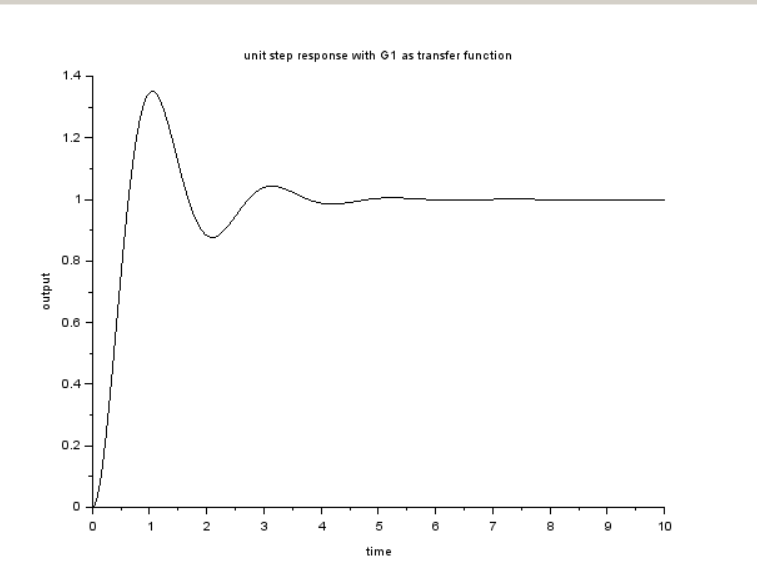
\includegraphics[width=0.98\textwidth]{transfer_function.png}
    \caption{Unit Step Response of the system with transfer function $G1(s)$}
    \label{fig:my_label}
\end{figure}
\subsection*{Scilab Code}
\begin{verbatim}
s = poly(0,'s');
G1 = 10/(s^2 + 2*s+10);
G2 = 5/(s+5);
//a) The equivalent transfer function is the product of two
G_cascade = G1*G2

// b) The equivalent transfer function is the addition of two
G_parallel = G1 + G2

// c) The equivalent transfer function is G1/(1+G1*G2) 
G_feedback = G1/(1+G1*G2)

// d) To find the output to step response we need to explicitly define G1 as a continuous time system using syslin command

G1 = syslin('c',G1);
t = 0:.01:10;         // for an total length of 10 units evaluated at intervals of .01
plot2d(t,csim('step',t,G1))    // csim returns a vector containing output on all values of t provided, with G1 as transfer function
xlabel('time')
ylabel('output')
title('unit step response with G1 as transfer function')
\end{verbatim}


\section*{Q2}
To find the poles and zeros, we can use the tf2zp function in Scilab.\\
 \begin{enumerate}
     \item Cascade system - Poles are $-5$,$-1+3i$,$-1-3i$. There are no zeros.\\
     \item Parallel system - Poles are $-5$,$-1+3i$,$-1-3i$. Zeros are $-2-4i$,$-2+4i$.\\
     \item Feedback system - Poles are $-6.3348$,$-0.3326+3.9592i$,$-0.3326-3.9592i$. Zeros are $-5$.\\
 \end{enumerate}
 \subsection*{Scilab Code}
 \begin{verbatim}
G_parallel = syslin('c',G_parallel);
G_cascade = syslin('c',G_cascade);
G_feedback = syslin('c',G_feedback);

// Poles and Zeroes of 
// 1. Cascade
[z_cascade, p_cascade, k] = tf2zp(G_cascade);

// 2. parallel
[z_parallel, p_parallel, k] = tf2zp(G_parallel);

// 1. Feedback
[z_feedback, p_feedback, k] = tf2zp(G_feedback);
 \end{verbatim}
 
 
\section*{Q3}
Applying Mesh Analysis on loop with current $I_1(s)$, we get
\begin{align*}
    \frac{2s^2+4s+3}{1+s}I_1 - \frac{I_2}{1+s} - (1+s)I_3 = 0\\
\end{align*}
Applying Mesh Analysis on loop with current $I_2(s)$, we get
\begin{align*}
    \frac{-I_1}{1+s} + \frac{s^2+4s+4}{1+s}I_2 - 2I_3 = 0\\
\end{align*}
Applying Mesh Analysis on loop with current $I_3(s)$, we get
\begin{align*}
    -(1+s)I_1 - 2I_2 + \frac{s^2+7s+7}{1+s}I_3 = v_1\\
\end{align*}
\begin{align*}
    \begin{bmatrix}
    -(1+s)&               -2 &               \frac{s^2+7s+7}{1+s}\\ 
      \frac{2s^2+4s+3}{1+s}& \frac{-1}{1+s}&          -(1+s)\\
     \frac{-1}{1+s}&             \frac{s^2+4s+4}{1+s}& -2\\
    \end{bmatrix} 
    \begin{bmatrix}
    I_1 \\ I_2 \\ I_3 \\
    \end{bmatrix}
    = \begin{bmatrix}
    V_1 \\ 0 \\ 0\\
    \end{bmatrix}\\
    Z(s) = \begin{bmatrix}
    -(1+s)&               -2 &               \frac{s^2+7s+7}{1+s}\\ 
      \frac{2s^2+4s+3}{1+s}& \frac{-1}{1+s}&          -(1+s)\\
     \frac{-1}{1+s}&             \frac{s^2+4s+4}{1+s}& -2\\
    \end{bmatrix} 
        \begin{bmatrix}
    I_1 \\ I_2 \\ I_3 \\
    \end{bmatrix} &= Y(s) \times \begin{bmatrix}
    V_1 \\ 0 \\ 0\\
    \end{bmatrix}\\
            \begin{bmatrix}
    I_1(s)/V_1(s) \\ I_2(s)/V_1(s) \\ I_3(s)/V_1(s) \\
    \end{bmatrix} &= Y(s)\times \begin{bmatrix}
    1 \\ 0 \\ 0\\
    \end{bmatrix}\\
\end{align*}
The transfer functions finally otained are\\
 \begin{enumerate}
     \item I1/V1 = $\frac{6+14s+13s^2+6s^3+s^4}{57 + 144s + 147s^2 + 74s^3 + 17s^4 + s^5}$\\
     \item I2/V1 = $\frac{7+16s+13s^2+4s^3}{57 + 144s + 147s^2 + 74s^3 + 17s^4 + s^5}$\\
     \item I3/V1 = $\frac{11+28s+27s^2+12s^3+2s^4}{57 + 144s + 147s^2 + 74s^3 + 17s^4 + s^5}$\\
 \end{enumerate}
\subsection*{Scilab Code}
\begin{verbatim}
Z = [-1-s,-2, (s^2+7*s+7)/(s+1); (2*s^2+ 4*s+3)/(s+1), -1/(s+1), -1-s; -1/(s+1), (s^2+4*s+4)/(s+1), -2];

Y = inv(Z);  // calculates inverse of Z
tf_vector = Y * [1;0;0]

// The final answers are
I1_V1 = tf_vector(1,1);
I2_V1 = tf_vector(2,1);
I3_V1 = tf_vector(3,1);
\end{verbatim}

\section*{Entire Code Snippet}
\begin{figure}[H]
    \centering
    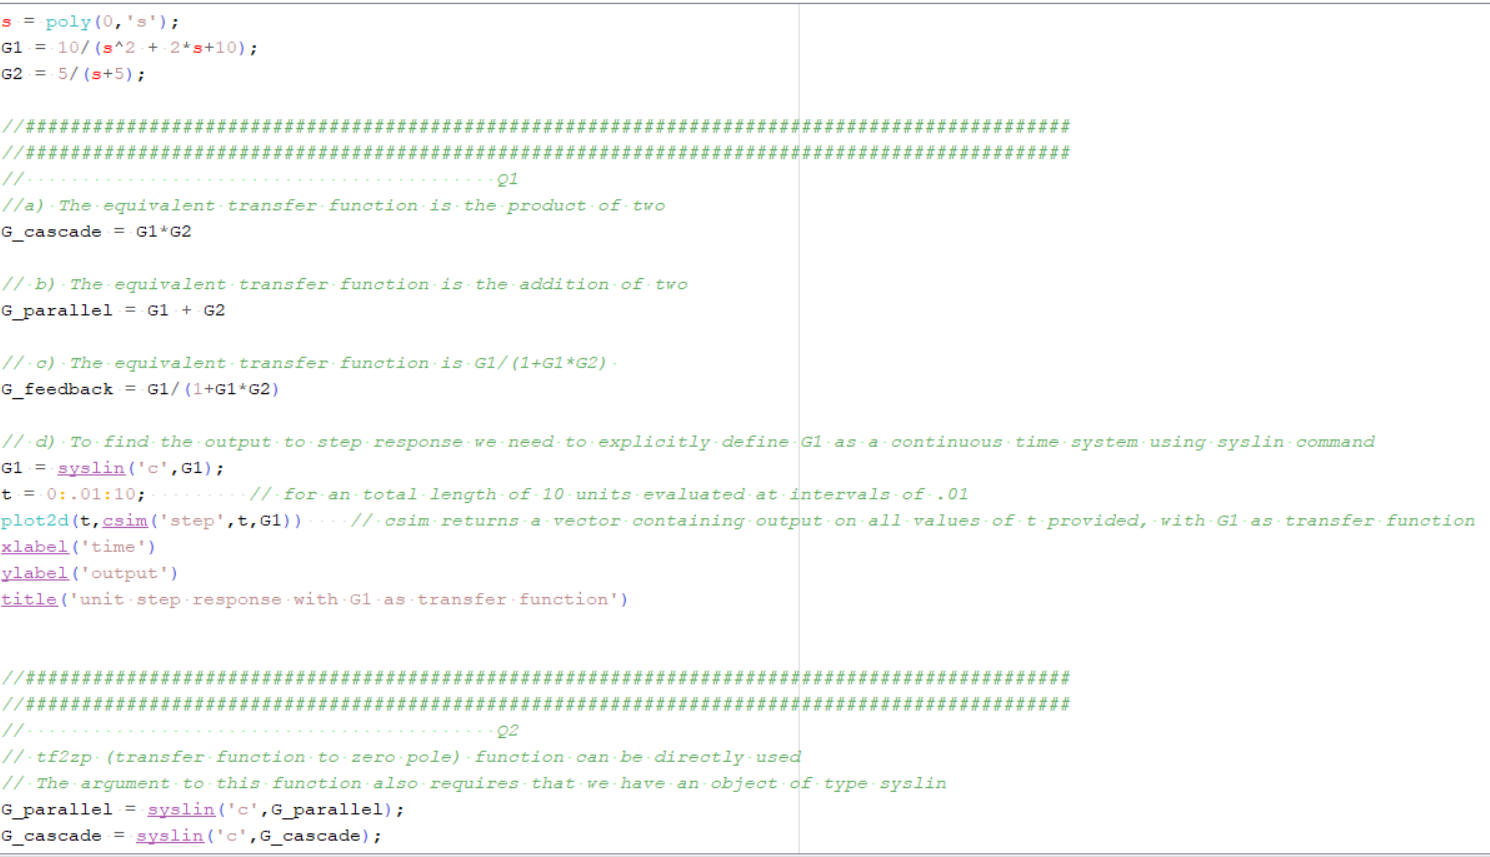
\includegraphics[width=0.98\textwidth]{snippet1.png}
\end{figure}
\begin{figure}[H]
    \centering
    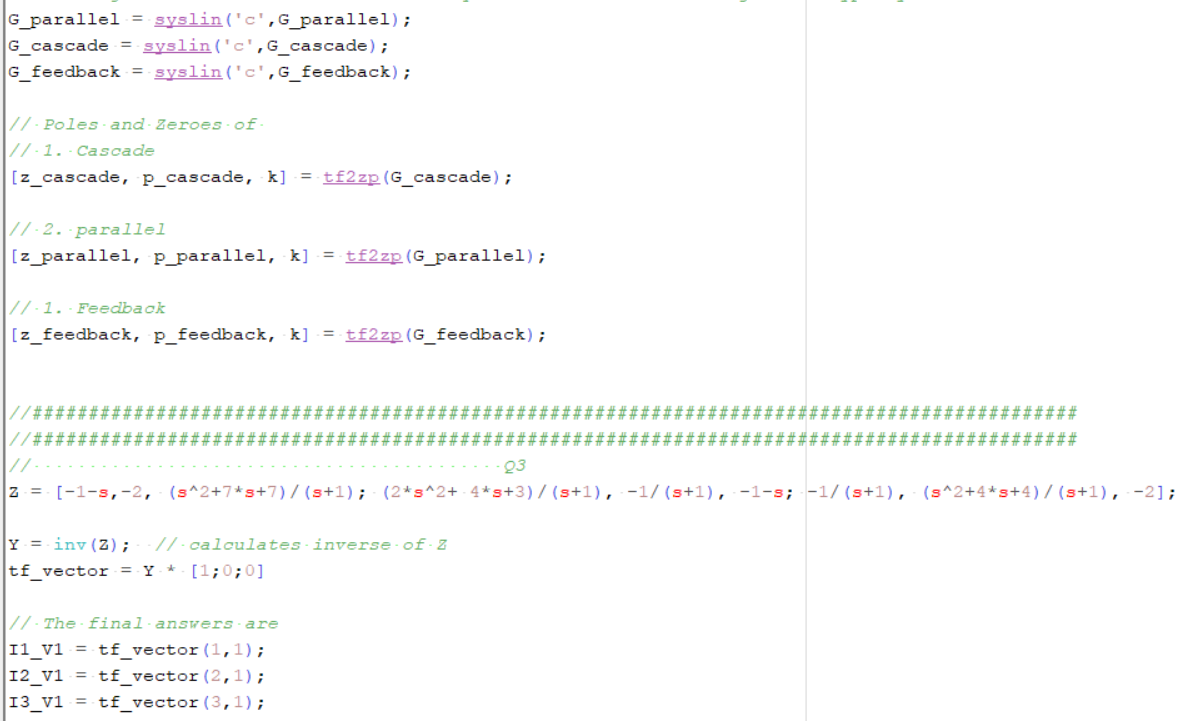
\includegraphics[width=0.98\textwidth]{snippet2.png}
    \caption{Entire  code snippet}
\end{figure}
\end{document}
